\graphicspath{{content/1_literatureReview/figures/}}
\section{DAC}\label{sec:dac}

\subsection{Configurations}

A DAC can be implemented using different summing op-amp configurations:
\begin{itemize}
    \item \textit{Inverting} vs \textit{Non-Inverting}. Single-supply inverting amplifiers require an offset bias at $V^+$ to keep the output positive.
          Non-inverting amplifiers suffer from input source coupling (discussed in Section \ref{dac_impedance}) and require a second stage to invert the output.
    \item \textit{Resistor-Weighted} vs \textit{R2R Ladder}. Resistor-weighted networks (RWN) use resistors continuously halving in value
          (e.g. in Figure \ref{fig:dac_nonInvertingRWN}). They are simple to build, but require large-valued precision resistors, or many parallel resistors.
          R2R Ladder networks (e.g in Figure \ref{fig:dac_invertingR2R}) solve this by re-using resistors across inputs.
\end{itemize}

\begin{figure}[!htb]
    \centering
    \begin{minipage}{.44\textwidth}
        \centering
        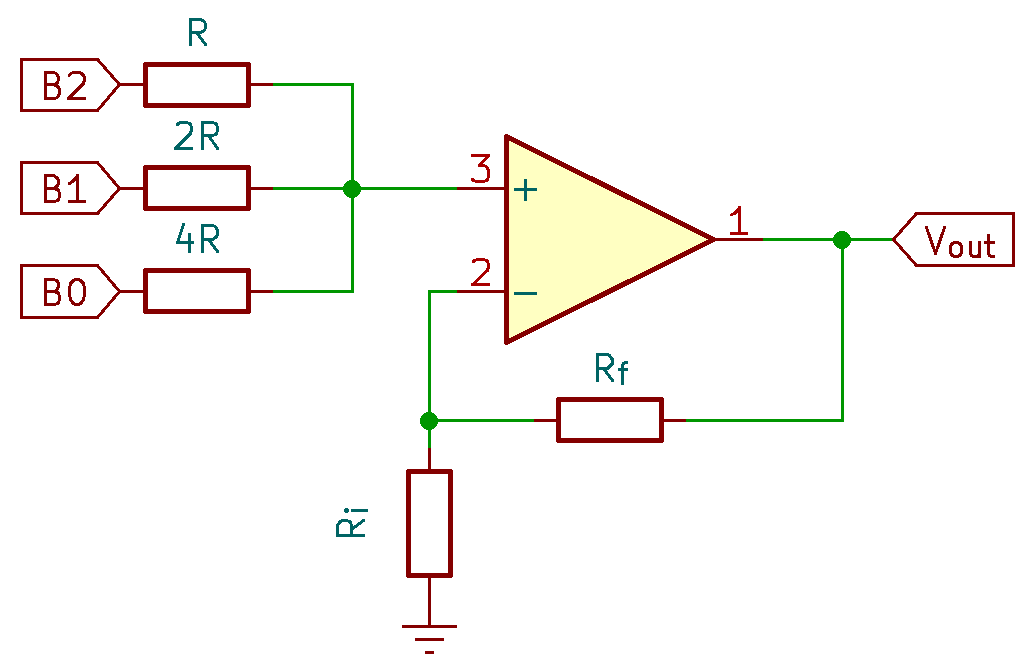
\includegraphics[width=0.7\linewidth]{dac_nonInvertingRWN}
        \captionof{figure}{Non-inverting mode with Resistor-Weighted Network \cite{SummingAmplifierBasics}}
        \label{fig:dac_nonInvertingRWN}
    \end{minipage}
    \begin{minipage}{.4\textwidth}
        \centering
        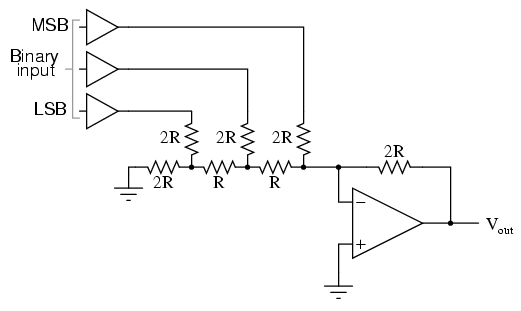
\includegraphics[width=0.9\linewidth]{dac_invertingR2R}
        \captionof{figure}{Inverting mode with R2R Ladder Network \cite{R2RDAC}}
        \label{fig:dac_invertingR2R}
    \end{minipage}
\end{figure}

Common-mode voltage range limitations should be considered. In inverting mode, $V^-$ is a "virtual ground" due to negative feedback.
This means common-mode voltage always equals the offset voltage at $V^+$. Rail voltage can therefore be chosen using only this voltage
and the output specifications. This is not true in non-inverting mode: the voltage at $V^+$ changes based on the source voltages.
For a DAC using the MCP6242, this means $V_{dd} \geq V_{digital} - 0.3 V$.

\subsection{Impedance}{\label{dac_impedance}}

For a practical source, $R_o \neq \SI{0}{\ohm}$, meaning amplifier input impedance should be considered. Non-inverting amplifiers do not have a "virtual ground",
meaning sources are not decoupled from each other \cite{SummingAmplifierBasics} causing some noise. Table \ref{tab:dac_amplifier_impedance} documents lowest input impedances:

\begin{table}[!h]
  \centering
  \renewcommand{\arraystretch}{1.2}
  \begin{tabular}{ |p{3cm}|p{6cm}|p{6cm}| }
    \hline
    \textbf{Configuration}         & \textbf{R2R}                               & \textbf{RWN}                      \\
    \hline
    \textbf{Inverting}             & 2R                                         & R                                 \\
    \hline
    \textbf{Non-Inverting}         & 4R                                         & $R \times \left(1 + \frac{1}{\frac{1}{2} + \frac{1}{4} + ... + \frac{1}{2^N}}\right) \approx 2R$                              \\
    \hline
  \end{tabular}
  \caption{Input impedance of various summing configurations}
  {\label{tab:dac_amplifier_impedance}}
\end{table}

\noindent For a practical load, $R_L \neq \infty$, meaning amplifier output impedance should be considered.
A buffer stage can be added. This lowers the output impedance of the op-amp.